\chapter{Alapvető definíciók ismertetése}

\section{Internet of Things}
Az IoT-ről, azaz a dolgok internetéről, akkor beszélhetünk, amikor az otthonunkban az internethez csatlakoztatott eszközök meghaladják az ott élő emberek számát. Ezeknek az eszközöknek a célja, hogy megkönnyítse mindennapi életünket, úgy, hogy egy digitális világban intelligens környezetet biztosít számunkra. intelligens eszközök segítségével adatgyűjtést végeznek a mindennapi tevékenységünkről, melyet továbbítják az úgynevezett felhőbe, hogy még precízebb képet tudjanak alkotni cselekvéseinkről. Az IoT eszközök nagyrészt vezeték nélkül csatlakoznak az internethez, mint például okos telefonok, okos otthonok és különböző az intelligens környezethez csatlakoztatható eszközök, a plug-in modulok.
\newline Az IoT 4 fő réteg szakaszból épül fel:\cite{smart-research}
\begin{itemize}
    \setlength\itemsep{-2pt}
    \item Észlelési réteg
    \item Hálózati réteg
    \item Közvetítői réteg
    \item Alkalmazási réteg 
\end{itemize}

\subsection{Smart Home}
Az intelligens otthon a technológia és a szolgáltatások integrálása az otthoni hálózatba. Rengeteg különböző technológiákat használ az otthon egyes részeinek felszerelésére az intelligensebb felügyelet és távvezérlés érdekében. A mindennapi háztartási feladatok és tevékenységek automatizálása anélkül, hogy a felhasználó beavatkozna abba.  Automatizáció implementálása a jobb életminőség érdekében. Bizonyos esetekben az otthoni szolgáltatások integrációja lehetővé teszi, hogy azok kommunikáljanak egymással az otthoni vezérlőn keresztül, ezáltal lehetővé téve, hogy egyetlen gomb segítségével különböző otthoni rendszereket vezéreljenek a mi fizikai beavatkozásunk nélkül.
\par Egy okosotthonban előre beprogramozott forgatókönyvek vagy működési módok, illetve tanulási minták alapján tervezett lépések vannak a rengeteg összegyűjtött szokási mintákból. Az intelligens otthonok javíthatják az otthoni kényelmet, komfortot, biztonságot és energiagazdálkodást. Ezen kívül az idősek és fogyatékkal élők számára is biztonságos és védett környezetet nyújthatnak.\cite{smart-home-technology}
\begin{figure}[!ht]
    \centering
    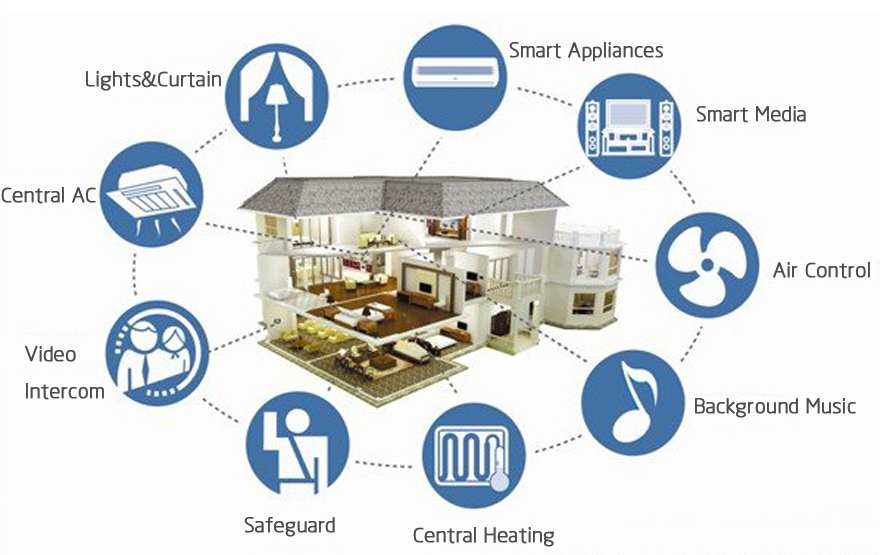
\includegraphics[width=70mm, keepaspectratio]{figures/smart-home.jpg}
    \caption{Okosotthon integrációs szolgáltatások}
\end{figure}
\par Rendkivűl pozitív előnye ennek a technológiának, hogy energiát és más erőforrásokat takarít meg. Az intelligens otthonok iránti fogyasztói lelkesedés ellenére azonban a biztonság és a védelem még mindig komoly aggodalomra ad okot. Ezek együttesen szabnak gátat a technológia elfogadásához.

\section{Biztonság}
Megállapíthatjuk, hogy a biztonság fogalma a civilizáció fejlődése során folyamatosan és exponenciálisan változik. Nehéz megfogalmazni, mivel nagyon komplex és számos területre ágaztathatjuk. Jogi biztonság, közlekedési, főként katonai és informatikai. A biztonságra való törekvés a történelem során mind az egyénben, mind a társadalomban jelen volt.
Az élet számos területein szükség van biztonsági intézkedésekre és azok elhárítására. Ma a katasztrófák vagy fenyegető vészhelyzetek olyan kihívások elé állítják a szakembereket, amelyek jellegükben, nagyságrendjükben és összetettségükben gyökeresen eltérnek a korábban tapasztaltaktól.\cite{kornyezetmernoki-tudastar} Ebben a szakdolgozatban az okosotthonok technologiájához kapcsolódó biztonsági intézkedéseket és azok sérülékenységeit fogom részletesen kifejteni és ismertetni.

\subsection{IT Security}
Ahogy a hackerek okosabbak és találékonyabbak lesznek, így még nagyobb az szükség van a digitális eszközök védelmére. Nagyrészt egy biztonságos rendszer kivitelezése költséges, de egy nem ismert biztonsági rés, jóval nagyobb pénzügyi kiesést tud okozni. A személyes adatok védelméhez informatikai biztonsági mechanizmusokra van szükség. Az IT security az információkat kezelő és tároló rendszereket, valamint az ezekbe történő feldolgozott adatokat védelmét fogalmazza meg. Az informatikai biztonságot gyakran a magánélet technikai oldalának tekintik. A biztonsági mechanizmusok belső mechanizmusok, amelyeket az informatikai rendszer valósít meg és külső mechanizmusok, amelyek a rendszeren kívül történnek. A témát öt fő részre taglalnák, amelyek közül kiemelném a hálózati biztonságot, ami lényegében megakadályozza, hogy illetéktelen felhasználók hozzáférhessenek egy hálózathoz. Ez a fajta biztonsági tényező biztosítja, hogy ne lehessen elérni az érzékeny és privát adatokat a hálózatokon keresztül.
\par Néhány szót ejtenék a végpontbiztonságról is, mely eszközszintű védelmet nyújt. A végpontbiztonság megakadályozza, hogy az eszközök hozzáférjenek a rosszindulatú hálózatokhoz, amelyek veszélyt jelenthetnek a felhasználók adataira. Naojain fejlett rosszindulatú programjaik elleni védelem és az eszközkezelő szoftverek példák a végpontbiztonságra. A végpontbiztonság által védett eszközök a táblagépek, mobiltelefonok, laptopok.
\par Tulajdonképpen minden olyan rendszerek, rendszerösszetevők, hálózati eszközök melyek alkalmasak adatok tárolására és továbbítására az IT Security fogalma alá tartoznak.\cite{cisco_2022}

\subsection{Cyber Security}
Alapesetben a kiberbiztonság a hálózatok és a rendszerek szoftveres biztonságát jelenti, számítógépekkel történő támadások ellen, viszont az elmúlt években a hálózatok a puszta kommunikációs eszközökből mindenütt jelenlévő számítástechnikai infrastrukturális hálózatokká alakultak át. A jelenlegi hálózatok nagyobbak, gyorsabbak és rendkívül dinamikusak. Ennek eredményeként a számítógépek és hálózati technológiák használata a kiberbiztonságot mára, már nemzetbiztonsági kérdéssé tette. Az internet a kormányok, vállalatok és a hétköznapi ember életének szerves része lett. A számítógépeket és a hálózatot például gyártási folyamatok kivitelezésére, tőzsdei rendszerek üzemeltetésére, légiforgalmi irányítási rendszerek kezelésére és a legújabb TikTok videó feltöltésére is használjuk. Az életünkbe való beépülés miatt a hálózati támadások elkezdték befolyásolni a valódi életünket is. Elsődleges célja egy kibertámadónak a pénzszerzés, melyet többféle módon is kivitelezhet. Célpont lehet közvetlenül egy kiszemelt bank, ami lássuk be nehezebben megvalósítható, viszont könnyebb préda egy ártatlan bankkártyafelhasználó. Különféle módok vannak a felhasználói adatok megszerzésére, amihez kizárólag a bankfiók tulajdonosát kell „meghackelni”, ezt nevezzük a Social Engineeringnek. Ebben az esetben az ember a kulcs és a gyenge láncszem. A felhasználóknak meg kell érteniük és be kellene tartaniuk olyan alapvető szabályokat és biztonsági előírásokat, mellyel megelőzhető lenne a személyes adataiknak a kiszivárgása. 
\par A digitális világban végrehajtott bűncselekményeket 3 fő csoportra oszthatjuk fel, ezek közül az elsőként említendő és a köztudatban a legelterjedtebb a kiberbűnözés, amely véghezvihető egyedül és csoportban is. Ezek a támadások legfőképpen pénzszerzés céljából alakulnak ki, a rendszer vagy hálózat sérülékenységeit kihasználva nyerészkednek, vagy kárt tesznek abban. 
\begin{figure}[!ht]
    \centering
    
\includegraphics[width=70mm, keepaspectratio]{figures/274638343_482850443543049_4683554889010609984_n.jpg}
    \caption{Anonymous hackercsoport szimbóluma}
\end{figure}
\par A kiberterror, az a jelenség, amikor a digitális világ adta előnyöket kihasználva információs infrastruktúrákat támadnak vagy ezen keresztül félemlítenek meg embereket, előre megfontolva ugyanúgy egyedül vagy csoportosan.
\par Az utolsó ismertetett fogalom a kiber támadás, amelynek általában a legfőbb célpontjai nagyobb csoportok, mint például egy ország vagy nemzet.\cite{cybersecurity}
